% Research defense slides — rebuilt from thesis Introduction and audited reports.
% Original Beamer theme, fonts, and color palette retained.
\documentclass[11pt]{beamer}
\usetheme{Hannover}
\usetheme{default}
\usepackage[utf8]{inputenc}
\usepackage{amsmath,amssymb,amsfonts}
\usepackage{graphicx}
\usepackage{caption}
\usepackage{booktabs}
\usepackage{tikz}
\usetikzlibrary{arrows.meta,positioning,shapes.geometric,calc,decorations.pathreplacing}
\definecolor{HN}{RGB}{35,60,85}
\definecolor{HT}{RGB}{30,119,130}
\definecolor{HG}{RGB}{99,108,117}
\newcommand{\subnote}[1]{\par\vspace{0.09cm}{\scriptsize\color{HG}#1\par}}
\newcommand{\keyidea}[1]{\vspace{0.12cm}\begin{center}\small\color{HN}\bfseries #1\end{center}}
\tikzset{
 module/.style={draw=HN!80,fill=HN!5,rounded corners=2pt,align=center,inner sep=5pt,font=\scriptsize},
 forecast/.style={draw=HT!90,fill=HT!9,rounded corners=2pt,align=center,inner sep=5pt,font=\scriptsize},
 neutral/.style={draw=HG!80,fill=HG!6,rounded corners=2pt,align=center,inner sep=5pt,font=\scriptsize},
 conn/.style={-{Latex[length=2mm]},thick,draw=HN!90}
}
\author{Dao Duy Hung}
\title{Learning Collaborative Action Policies for Humans and Robots with Intent Awareness}
\institute{Research in Human--Robot Collaboration}
\date{November 2026}
\setbeamertemplate{caption}[numbered]
\setbeamertemplate{footline}[frame number]
\tikzset{
 stage/.style={draw=HN!80,fill=HN!5,rounded corners=2pt,align=center,inner sep=4.5pt,font=\scriptsize},
 future/.style={draw=HT!80,fill=HT!9,rounded corners=2pt,align=center,inner sep=4.5pt,font=\scriptsize},
 axis/.style={->,thick,draw=HN}
}

\graphicspath{{../../reports/bao_cao_2026-10-25/fig/}{../../slides/tien_do_2026-10-06/figures/}{../../slides/bao_cao_2026-10-18/figures/}}
\begin{document}
\begin{frame}
\titlepage
\end{frame}

\begin{frame}{Introduction \hfill Timely coordination in HRC}
\centering
\begin{tikzpicture}[font=\scriptsize,>=Latex]
\foreach \x/\name/\caption in {
-3.57/c1_A_t40.png/{Human action},
-1.16/c1_A_t80.png/{Robot readiness},
1.25/c1_A_t96.png/{Interaction}
}{
\node[draw=HG!35,inner sep=2pt] at (\x,1.31)
 {\includegraphics[width=2.08cm,height=1.47cm,keepaspectratio]{\name}};
\node[font=\scriptsize,align=center] at (\x,0.12){\caption};
}
\node[draw=HG!40,fill=HG!7,minimum width=2.05cm,minimum height=1.5cm] at (3.67,1.31) {};
\draw[very thick,HT] (3.19,1.30)--(3.53,0.97)--(4.15,1.83);
\node[font=\scriptsize] at (3.67,0.12){Task completion};
\draw[->,thick,HN] (-4.65,-0.39)--(4.7,-0.39);
\foreach \x in {-3.57,-1.16,1.25,3.67}{\fill[HT] (\x,-0.39) circle (2.4pt);}
\end{tikzpicture}
\vspace{0.18cm}
\keyidea{Effective HRC requires correct, timely and closely coordinated robot responses.}
\end{frame}

\begin{frame}{Introduction \hfill Why imitation learning?}
\centering
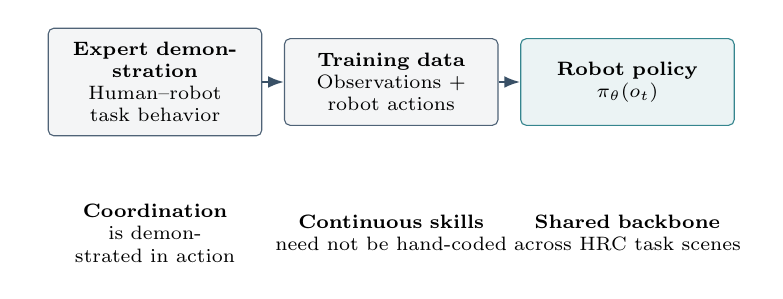
\begin{tikzpicture}[font=\scriptsize,>=Latex]
\node[module,text width=2.36cm,minimum height=1.10cm] (a) at (-3,1.45)
 {\textbf{Expert demonstration}\\Human--robot task behavior};
\node[module,text width=2.36cm,minimum height=1.10cm] (b) at (0,1.45)
 {\textbf{Training data}\\Observations + robot actions};
\node[forecast,text width=2.36cm,minimum height=1.10cm] (c) at (3,1.45)
 {\textbf{Robot policy}\\$\pi_\theta(o_t)$};
\draw[conn] (a)--(b); \draw[conn] (b)--(c);
\node[align=center,text width=3.0cm] at (-3,-0.47)
 {\textbf{Coordination}\\is demonstrated in action};
\node[align=center,text width=3.0cm] at (0,-0.47)
 {\textbf{Continuous skills}\\need not be hand-coded};
\node[align=center,text width=3.0cm] at (3,-0.47)
 {\textbf{Shared backbone}\\across HRC task scenes};
\end{tikzpicture}
\keyidea{Imitation learning can acquire manipulation and coordination from expert behavior.}
\end{frame}

\begin{frame}{Introduction \hfill Why intent awareness?}
\centering
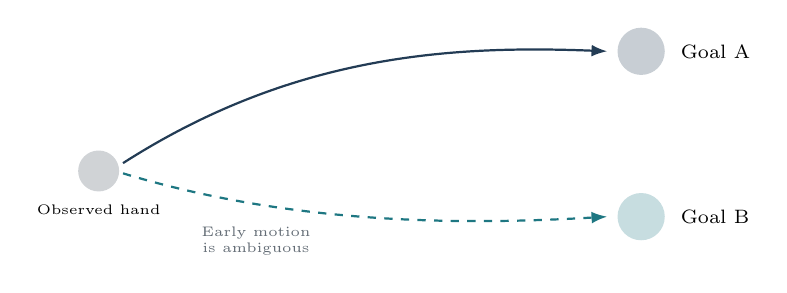
\begin{tikzpicture}[font=\scriptsize,>=Latex]
\fill[HG!30] (-3.55,0.1) circle (0.26);
\node[below,font=\tiny] at (-3.55,-0.21){Observed hand};
\fill[HN!25] (3.34,1.62) circle (0.30);
\fill[HT!25] (3.34,-0.48) circle (0.30);
\node[right] at (3.72,1.62){Goal A};
\node[right] at (3.72,-0.48){Goal B};
\draw[-{Latex[length=2mm]},HN,thick] (-3.24,0.2)..controls (-1.1,1.57) and (0.9,1.7)..(2.91,1.62);
\draw[-{Latex[length=2mm]},HT,thick,dashed] (-3.24,0.07)..controls (-1.2,-0.55) and (0.9,-0.6)..(2.91,-0.48);
\node[font=\tiny,HG,align=center] at (-1.55,-0.79){Early motion\\is ambiguous};
\end{tikzpicture}
\vspace{0.18cm}
\begin{columns}[T]
\column{.47\textwidth}\centering\small \textbf{Observed behavior}\\May be insufficient for early action
\column{.47\textwidth}\centering\small \textbf{Predicted behavior}\\Can guide preparation before full reveal
\end{columns}
\keyidea{The robot must use predicted intent without assuming the prediction is always correct.}
\end{frame}

\begin{frame}{Related Work \hfill Forecasting and action learning address different layers}
\centering\scriptsize
\renewcommand{\arraystretch}{1.53}
\begin{tabular}{p{2.18cm}p{2.88cm}p{3.75cm}}
\toprule
\textbf{Work} & \textbf{Relevant approach} & \textbf{Relevance to this thesis}\\
\midrule
Hoffman (2007, 2019) & Anticipatory teamwork; fluency & Temporal coordination is part of collaboration\\
ManiCast (CoRL 2023) & Cost-aware human forecasts + MPC & Predicts future human motion for robot decisions\\
ACT (RSS 2023) & Imitation of continuous action chunks & Robot manipulation policy backbone\\
Diffusion Co-Policy (RA-L 2024) & Learn coordinated human--robot action sequences & Human motion may condition learned collaboration\\
Learning to Assist (2026) & Learned assistance from implicit cues & Anticipatory timing remains a learning question\\
\bottomrule
\end{tabular}
\vspace{0.21cm}
\begin{center}\small\bfseries
Research focus: how predicted human motion influences a learned robot policy.
\end{center}

\end{frame}

\begin{frame}{Our Proposal \hfill Intent-aware imitation learning for HRC}
\centering
\[
\boxed{\quad \pi_\theta(o_t,\hat H_t)\ \rightarrow\ \hat A_{t:t+H-1}\quad}
\]
\begin{center}\scriptsize
$o_t$: current observations \qquad $\hat H_t$: forecast human poses\\
$\pi_\theta$: ACT action policy \qquad $\hat A_{t:t+H-1}$: robot action chunk
\end{center}
\vspace{.13cm}
\begin{enumerate}\small\setlength{\itemsep}{.24cm}
\item \textbf{Claim 1 -- Anticipatory coordination:} reduce unnecessary waiting and task completion time.
\item \textbf{Claim 2 -- Intent adaptability:} handle inaccurate predictions and changes in human goals.
\item \textbf{Benchmark contribution:} multi-task simulated HRC with quantitative evaluation.
\end{enumerate}
\end{frame}

\begin{frame}{Proposed Method \hfill Overall system architecture}
\centering
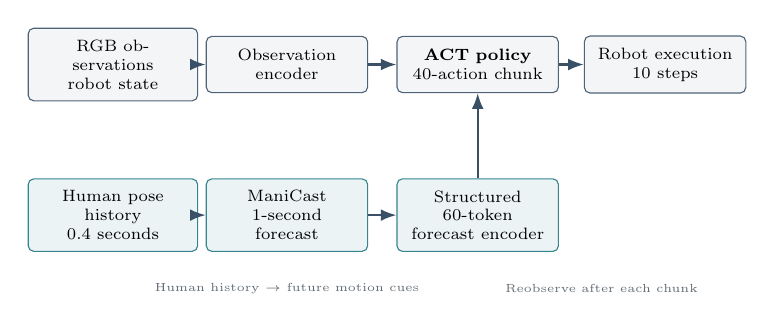
\begin{tikzpicture}[font=\scriptsize,>=Latex,scale=0.85,transform shape]
\node[module,text width=2.18cm,minimum height=.84cm] (scene) at (-4.1,2.0){RGB observations\\robot state};
\node[module,text width=2.06cm,minimum height=.84cm] (vis) at (-1.5,2.0){Observation\\encoder};
\node[module,text width=2.06cm,minimum height=.84cm] (act) at (1.35,2.0){\textbf{ACT policy}\\40-action chunk};
\node[module,text width=2.06cm,minimum height=.84cm] (exec) at (4.15,2.0){Robot execution\\10 steps};
\node[forecast,text width=2.18cm,minimum height=.84cm] (hist) at (-4.1,-.25){Human pose history\\0.4 seconds};
\node[forecast,text width=2.06cm,minimum height=.84cm] (man) at (-1.5,-.25){ManiCast\\1-second forecast};
\node[forecast,text width=2.06cm,minimum height=.84cm] (tok) at (1.35,-.25){Structured 60-token\\forecast encoder};
\draw[conn] (scene.east)--(vis.west);
\draw[conn] (vis.east)--(act.west);
\draw[conn] (act.east)--(exec.west);
\draw[conn] (hist.east)--(man.west);
\draw[conn] (man.east)--(tok.west);
\draw[conn] (tok.north)--(act.south);
\node[font=\tiny,HG] at (-1.5,-1.34){Human history $\to$ future motion cues};
\node[font=\tiny,HG] at (3.20,-1.34){Reobserve after each chunk};
\end{tikzpicture}
\begin{center}\scriptsize
Two observation streams condition the same ACT policy. Connections terminate at module boundaries.
\end{center}
\end{frame}

\begin{frame}{Proposed Method \hfill Structured future-motion representation}
\centering
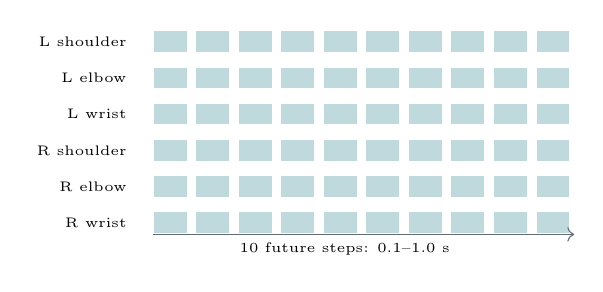
\begin{tikzpicture}[font=\scriptsize,x=.54cm,y=.46cm]
\foreach \r/\lab in {0/{L shoulder},1/{L elbow},2/{L wrist},3/{R shoulder},4/{R elbow},5/{R wrist}}{
\node[anchor=east,font=\tiny] at (-.4,5-\r){\lab};
\foreach \c in {0,...,9}{\filldraw[fill=HT!28,draw=white] (\c,4.7-\r) rectangle (\c+.8,5.3-\r);}
}
\draw[->,HG] (0,-.32)--(9.9,-.32);
\node[font=\tiny] at (4.5,-.72){10 future steps: 0.1--1.0 s};
\end{tikzpicture}
\[
\hat H_t\in\mathbb R^{10\times6\times3},\qquad
z_{k,j}=\mathrm{LN}\big(W[x_{k,j},v]+e_k^{\mathrm{time}}+e_j^{\mathrm{joint}}\big)
\]
\begin{center}\scriptsize
$k$: future time; $j$: body joint; $\hat H_t$: forecasted 3D poses.\\
$x_{k,j}$: position, TCP-relative displacement and velocity; $v$: validity flag.\\
$e^{\mathrm{time}},e^{\mathrm{joint}}$: embeddings; $z_{k,j}$: forecast token for ACT.
\end{center}
\end{frame}

\begin{frame}{Proposed Method \hfill The training signal must reach the forecast encoder}
\centering
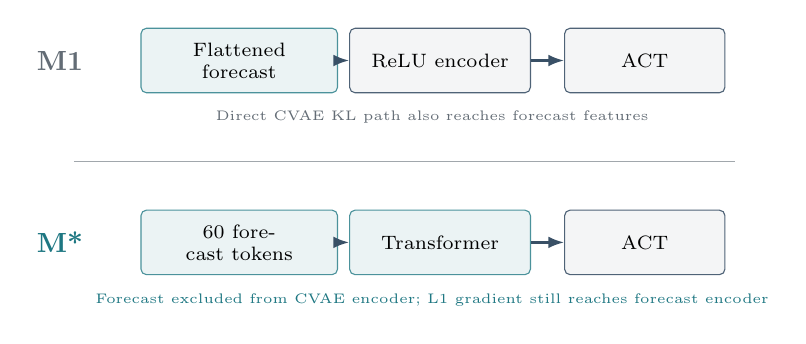
\begin{tikzpicture}[font=\scriptsize,>=Latex]
\node[anchor=east,font=\bfseries,HG] at (-3.96,2.49){M1};
\node[future,text width=2.18cm,minimum height=0.82cm] (f) at (-2.1,2.49){Flattened forecast};
\node[stage,text width=1.98cm,minimum height=0.82cm] (relu) at (0.45,2.49){ReLU encoder};
\node[stage,text width=1.72cm,minimum height=0.82cm] (act) at (3.05,2.49){ACT};
\draw[conn] (f)--(relu);\draw[conn] (relu)--(act);
\node[below,font=\tiny,HG] at (0.35,1.98){Direct CVAE KL path also reaches forecast features};
\draw[HG!60] (-4.2,1.21)--(4.20,1.21);
\node[anchor=east,font=\bfseries,HT] at (-3.96,0.18){M*};
\node[future,text width=2.18cm,minimum height=0.82cm] (sf) at (-2.1,0.18){60 forecast tokens};
\node[future,text width=1.98cm,minimum height=0.82cm] (st) at (0.45,0.18){Transformer};
\node[stage,text width=1.72cm,minimum height=0.82cm] (ac) at (3.05,0.18){ACT};
\draw[conn] (sf)--(st);\draw[conn] (st)--(ac);
\node[below,font=\tiny,HT,align=center] at (0.35,-0.35){Forecast excluded from CVAE encoder; L1 gradient still reaches forecast encoder};
\end{tikzpicture}

\end{frame}

\begin{frame}{Proposed Method \hfill Decision-aware imitation learning}
\[
\boxed{\quad \mathcal L =
\frac{\sum_i w_i\ell_{\mathrm{L1},i}}{\sum_i w_i}
+10\,\mathcal L_{\mathrm{KL}},
\qquad w_i=1+2m_i\quad}
\]
\centering
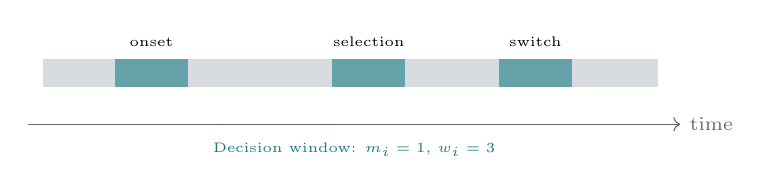
\begin{tikzpicture}[font=\scriptsize,x=.92cm,y=.80cm]
\draw[->,HG] (0,0)--(9.0,0) node[right]{time};
\fill[HN!18] (.2,.6) rectangle (8.7,1.04);
\foreach \a/\b in {1.2/2.2,4.2/5.2,6.5/7.5}{\fill[HT!69] (\a,.6) rectangle (\b,1.04);}
\node[above,font=\tiny] at (1.7,1.08){onset};
\node[above,font=\tiny] at (4.7,1.08){selection};
\node[above,font=\tiny] at (7.0,1.08){switch};
\node[font=\tiny,HT] at (4.5,-.40){Decision window: $m_i=1$, $w_i=3$};
\end{tikzpicture}
\begin{center}\scriptsize
$\ell_{\mathrm{L1},i}$: demonstration-versus-prediction error for action chunk $i$.\\
$m_i$: event-window indicator; $w_i$: training-sample weight.\\
$\mathcal L_{\mathrm{KL}}$: ACT latent regularization; $10$: KL coefficient.
\end{center}
\end{frame}

\begin{frame}{Simulated Benchmark \hfill Tasks grouped by research claim}
\centering\scriptsize
\renewcommand{\arraystretch}{1.55}
\begin{tabular}{p{1.25cm}p{2.14cm}p{2.55cm}p{2.39cm}}
\toprule
\textbf{Objective} & \textbf{Interaction type} & \textbf{Scenes / conditions} & \textbf{Evaluation focus}\\
\midrule
Claim 1 & Cooperative & C1, C2, C3 & Coordination and completion time\\
Claim 1 & Human-guided & I1, I2, I3 nominal & Responsive action and success\\
Claim 1 & Concurrent work & W1, W1 linger, W2 & Task-general performance\\
\midrule
Claim 2 & Goal switching & I3 switch-before & Adaptation before commitment\\
Claim 2 & Goal switching & I3 switch-after & Adaptation after commitment\\
\bottomrule
\end{tabular}
\vspace{.23cm}
\begin{columns}[T,onlytextwidth]
\column{.50\textwidth}\centering
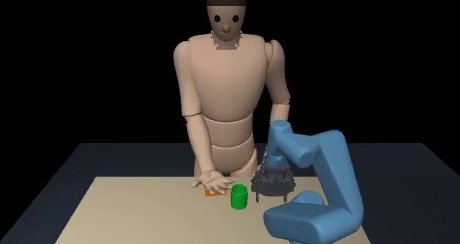
\includegraphics[width=3.8cm,height=1.35cm,keepaspectratio]{c1_A_t80.png}
{\scriptsize Cooperative task}
\column{.50\textwidth}\centering
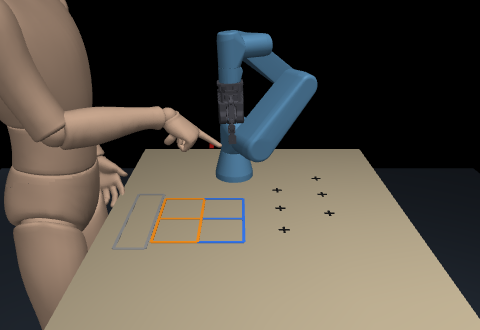
\includegraphics[width=3.8cm,height=1.35cm,keepaspectratio]{point.png}
{\scriptsize Human-guided task}
\end{columns}
\end{frame}

\begin{frame}{Benchmark \hfill Metrics organized by evaluation objective}
\centering\scriptsize
\renewcommand{\arraystretch}{1.46}
\begin{tabular}{p{2.05cm}p{1.31cm}p{4.86cm}}
\toprule
\textbf{Objective} & \textbf{Metric} & \textbf{Definition}\\
\midrule
Claim 1: efficiency & CT $\downarrow$ & Mean task completion time on successful runs\\
Claim 1: timeliness & Rsp $\downarrow$ & Response latency after relevant human action\\
Completion & CSR $\uparrow$ & Fraction of successful episodes\\
Task progress & OC $\uparrow$ & Fraction of expected steps completed\\
Contact behavior & CFR $\uparrow$ & Contact-free episode rate under project definition\\
\midrule
Claim 2: adaptation & Switch CSR & Completion following goal changes\\
Coordination & TSync / DSR & Event synchronization / disruption recovery\\
\bottomrule
\end{tabular}
\begin{center}\scriptsize
Metrics follow project-defined evaluation rules; unavailable measurements are denoted n/a.
\end{center}
\end{frame}

\begin{frame}{Evaluation \hfill Paired observations, shared seeds, fixed checkpoints}
\centering
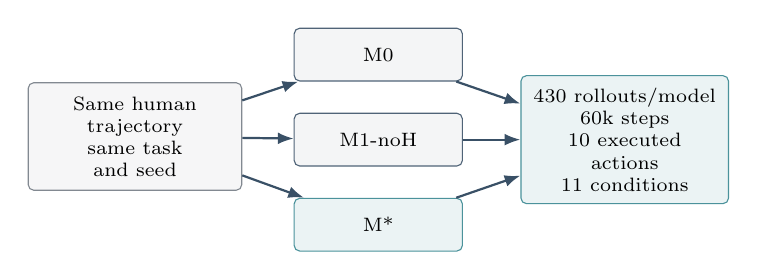
\begin{tikzpicture}[font=\scriptsize,>=Latex]
\node[neutral,text width=2.36cm,minimum height=1.20cm] (seed) at (-3.12,1.52){Same human trajectory\\same task and seed};
\node[stage,text width=1.82cm,minimum height=0.67cm] (m0) at (-0.03,2.56){M0};
\node[stage,text width=1.82cm,minimum height=0.67cm] (mn) at (-0.03,1.48){M1-noH};
\node[future,text width=1.82cm,minimum height=0.67cm] (ms) at (-0.03,0.40){M*};
\node[future,text width=2.32cm,minimum height=1.48cm] (out) at (3.10,1.48){430 rollouts/model\\60k steps\\10 executed actions\\11 conditions};
\draw[conn] (seed)--(m0);\draw[conn] (seed)--(mn);\draw[conn] (seed)--(ms);
\draw[conn] (m0)--(out);\draw[conn] (mn)--(out);\draw[conn] (ms)--(out);
\end{tikzpicture}
\keyidea{1,290 matched validation rollouts; not an independent test set.}

\end{frame}

\begin{frame}{Results \hfill Macro mean across 11 conditions}
\centering\vspace{.09cm}
\resizebox{.98\textwidth}{!}{%
\begin{tabular}{lcrrrrrrr}
\toprule
\textbf{Model} & \textbf{Cond.} & \textbf{CSR $\uparrow$} & \textbf{CT (s) $\downarrow$} & \textbf{Rsp (s) $\downarrow$} & \textbf{OC $\uparrow$} & \textbf{CFR $\uparrow$} & \textbf{DSR} & \textbf{TSync $\uparrow$}\\
\midrule
M0 & 11 & 0.73 & 21.23 & 0.31 & 0.77 & 0.93 & n/a & 1.00\\
M1-noH & 11 & 0.60 & 19.19 & \textbf{0.28} & 0.67 & 0.97 & n/a & 0.91\\
\textbf{\color{HT}Ours (M*)} & \textbf{11} & \textbf{0.77} & \textbf{19.02} & 0.30 & \textbf{0.78} & \textbf{0.98} & n/a & 0.93\\
\bottomrule
\end{tabular}}
\vspace{.33cm}
\begin{center}\small
Macro mean: each condition contributes equally.\\[6pt]
\scriptsize CSR, CT, OC, CFR: 11 conditions; Rsp: 7; TSync: 6; DSR: 0.
\end{center}
\vspace{.10cm}
\begin{center}\small
Ours leads on macro CSR, CT and CFR, but M1-noH has the lowest mean response latency.
\end{center}
\end{frame}

\begin{frame}{Claim 1 \hfill Efficiency and timely robot response}
\centering
\begin{columns}[T]
\column{.5\textwidth}\centering
{\scriptsize\bfseries Completion time, macro mean (s)}
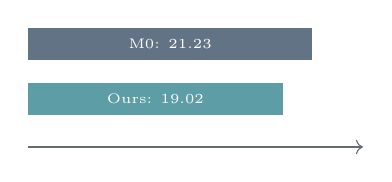
\begin{tikzpicture}[font=\tiny,x=.17cm,y=.75cm]
\draw[->,HG] (0,0)--(25,0);
\fill[HN!72] (0,1.48) rectangle (21.23,2.02);
\fill[HT!72] (0,.54) rectangle (19.02,1.08);
\node[white] at (10.6,1.75){M0: 21.23};
\node[white] at (9.5,.81){Ours: 19.02};
\end{tikzpicture}
\column{.5\textwidth}\centering
{\scriptsize\bfseries Response latency, macro mean (s)}
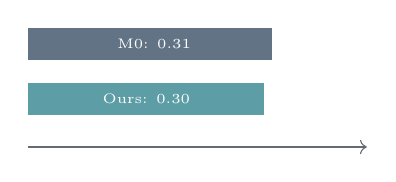
\begin{tikzpicture}[font=\tiny,x=10cm,y=.75cm]
\draw[->,HG] (0,0)--(.43,0);
\fill[HN!72] (0,1.48) rectangle (.31,2.02);
\fill[HT!72] (0,.54) rectangle (.30,1.08);
\node[white] at (.16,1.75){M0: 0.31};
\node[white] at (.15,.81){Ours: 0.30};
\end{tikzpicture}
\end{columns}
\vspace{.32cm}
\scriptsize\centering
\renewcommand{\arraystretch}{1.36}
\begin{tabular}{lrrrr}
\toprule
& \multicolumn{2}{c}{\textbf{CT (s)}} & \multicolumn{2}{c}{\textbf{Rsp (s)}}\\
Condition & M0 & Ours & M0 & Ours\\
\midrule
C1 & 24.9 & 21.2 & 0.26 & 0.22\\
I1 & 24.3 & 22.1 & 0.57 & 0.08\\
\bottomrule
\end{tabular}
\vspace{.12cm}
\begin{center}\scriptsize
Macro CT is 2.21 s lower for Ours; temporal effects vary by task. CT includes successful episodes only.
\end{center}
\end{frame}

\begin{frame}{Claim 2 \hfill Behavior when human goals change}
\centering
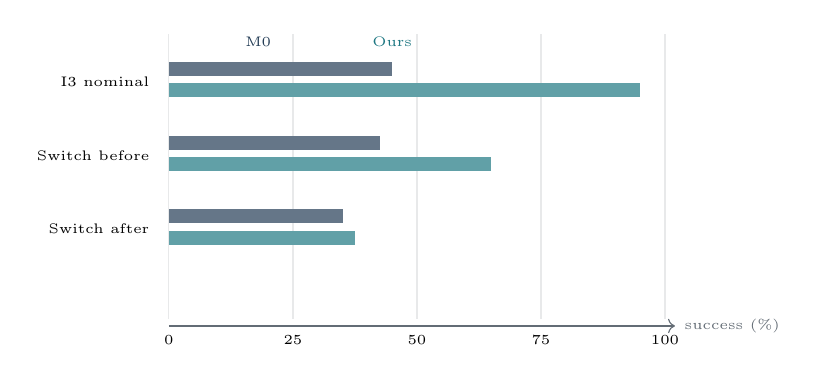
\begin{tikzpicture}[font=\scriptsize,x=.063cm,y=.78cm]
\draw[->,HG] (0,0)--(102,0) node[right,font=\tiny]{success (\%)};
\foreach \v in {0,25,50,75,100}{\draw[HG!15] (\v,.12)--(\v,4.75);\node[below,font=\tiny] at (\v,0){\v};}
\node[anchor=east,font=\tiny] at (-2,3.98){I3 nominal};
\node[anchor=east,font=\tiny] at (-2,2.78){Switch before};
\node[anchor=east,font=\tiny] at (-2,1.58){Switch after};
\fill[HN!70] (0,4.07) rectangle (45,4.3);
\fill[HT!70] (0,3.72) rectangle (95,3.95);
\fill[HN!70] (0,2.87) rectangle (42.5,3.1);
\fill[HT!70] (0,2.52) rectangle (65,2.75);
\fill[HN!70] (0,1.67) rectangle (35,1.9);
\fill[HT!70] (0,1.32) rectangle (37.5,1.55);
\node[font=\tiny,HN] at (18,4.63){M0};
\node[font=\tiny,HT] at (45,4.63){Ours};
\end{tikzpicture}
\vspace{.13cm}
\begin{center}\scriptsize
40 paired seeds per condition. McNemar: nominal $p<.001$; before $p=.078$; after $p=1.00$.
\end{center}
\vspace{.12cm}
\begin{center}\small
Nominal improvement is strong; post-commit recovery is not established.
\end{center}
\end{frame}

\begin{frame}{Conclusion \hfill Intent-aware imitation learning for HRC}
\vspace{.15cm}
\begin{enumerate}\setlength{\itemsep}{.34cm}
\item \textbf{Framework:} structured ManiCast forecasts condition a unified ACT policy trained from demonstrations.
\item \textbf{Claim 1:} mean task completion time decreases; responsiveness gains are task-dependent.
\item \textbf{Claim 2:} adaptation results vary with the timing of human goal changes.
\item \textbf{Benchmark:} physically constrained HRC simulation enables task, timing and adaptation comparisons.
\end{enumerate}
\vspace{.17cm}
\keyidea{Learning to use predicted human motion is a path toward timely and adaptive collaboration.}
\end{frame}
\end{document}
